% =====================================================================
% Skeleton F — 4 Phase Horizontal + Multi Vertical Sub-elements per Phase
% =====================================================================
% USAGE: Adapted from a GOLD STANDARD figure (Privacy-Preserving MPC
% Protocol). Sub-agent: copy ENTIRE file as figure.tex, change content.
%
% LAYOUT MODEL:
%   ┌───────────┬───────────┬───────────┬───────────┐
%   │ Phase 1   │ Phase 2   │ Phase 3   │ Phase 4   │
%   │  Setup    │  Encrypt  │  Compute  │  Output   │
%   │ ┌───────┐ │ ┌───────┐ │ ┌───────┐ │ ┌───────┐ │
%   │ │ Sub-1 │ │ │Party A│ │ │ Hero  │ │ │ Recv  │ │
%   │ │ Sub-2 │ │ │Party B│ │ │ Multi │ │ │  ZK   │ │
%   │ │ Sub-3 │ │ │Party C│ │ │ layer │ │ │  Perf │ │
%   │ └───────┘ │ └───────┘ │ └───────┘ │ └───────┘ │
%   └───────────┴───────────┴───────────┴───────────┘
%   Each phase = container with 3+ vertical sub-elements inside.
%
% WHEN TO USE: Multi-party protocols (MPC, threshold sig), staged
% systems with internal sub-elements per stage (vs single hero per stage).
%
% CONTAINS: 4 phase containers + Phase 1 (3 setup sub-blocks) + Phase 2
% (3 parallel parties) + Phase 3 (Garbled Circuit + OT + Eval hero) +
% Phase 4 (Output Recovery + ZK Verification + Performance bar).
% =====================================================================

\documentclass[tikz,border=25pt]{standalone}
\usepackage{tikz}
\usepackage[fontset=none]{ctex}
\setCJKmainfont{PingFang SC}
\setCJKsansfont{PingFang SC}
\usepackage{amsmath,amssymb}
\usetikzlibrary{shapes, arrows.meta, positioning, fit, backgrounds, calc, shadows, shapes.geometric}

% ===== 学术配色（新默认） =====
\definecolor{acaBlueLine}{HTML}{6080B0}      \definecolor{acaBlueFill}{HTML}{DBEAFE}
\definecolor{acaGreenLine}{HTML}{30A060}     \definecolor{acaGreenFill}{HTML}{A0D0A0}
\definecolor{acaOrangeLine}{HTML}{D06020}    \definecolor{acaOrangeFill}{HTML}{FFE6CC}
\definecolor{acaPurpleLine}{HTML}{6020D0}    \definecolor{acaPurpleFill}{HTML}{E1D5E7}
\definecolor{acaRedLine}{HTML}{B05050}       \definecolor{acaRedFill}{HTML}{F8CECC}
\definecolor{acaGreyLine}{HTML}{666666}      \definecolor{acaGreyFill}{HTML}{F5F5F5}
\definecolor{acaGoldLine}{HTML}{D09000}      \definecolor{acaGoldFill}{HTML}{F8F8E0}
\definecolor{acaTealLine}{HTML}{009060}      \definecolor{acaTealFill}{HTML}{D1FAE5}
\definecolor{acaCyanLine}{HTML}{00B0D0}      \definecolor{acaCyanFill}{HTML}{E0F7FA}
\definecolor{acaPinkLine}{HTML}{D06090}      \definecolor{acaPinkFill}{HTML}{FCE4EC}
\definecolor{acaYellowLine}{HTML}{E0C060}    \definecolor{acaYellowFill}{HTML}{FFF8E1}
\definecolor{acaLimeLine}{HTML}{80B060}      \definecolor{acaLimeFill}{HTML}{E8F5E9}
% Zone 背景
\definecolor{zoneBlueBg}{HTML}{E0E0F8}
\definecolor{zoneGreenBg}{HTML}{ECFDF5}
\definecolor{zonePurpleBg}{HTML}{F5F3FF}
\definecolor{zoneRedBg}{HTML}{F8E0E0}
\definecolor{zoneYellowBg}{HTML}{F8F0C0}
% 热力图
\definecolor{heatDeep}{HTML}{401090}
\definecolor{heatDark}{HTML}{6020D0}
\definecolor{heatMid}{HTML}{8B5CF6}
\definecolor{heatLight}{HTML}{C4B5FD}
\definecolor{heatBg}{HTML}{EDE9FE}
% 数据图表
\definecolor{barBlue}{HTML}{3080C0}
\definecolor{barGreen}{HTML}{30A060}
\definecolor{barOrange}{HTML}{D06020}
\definecolor{barRed}{HTML}{E03030}

\pgfdeclarelayer{background}
\pgfsetlayers{background,main}

\begin{document}
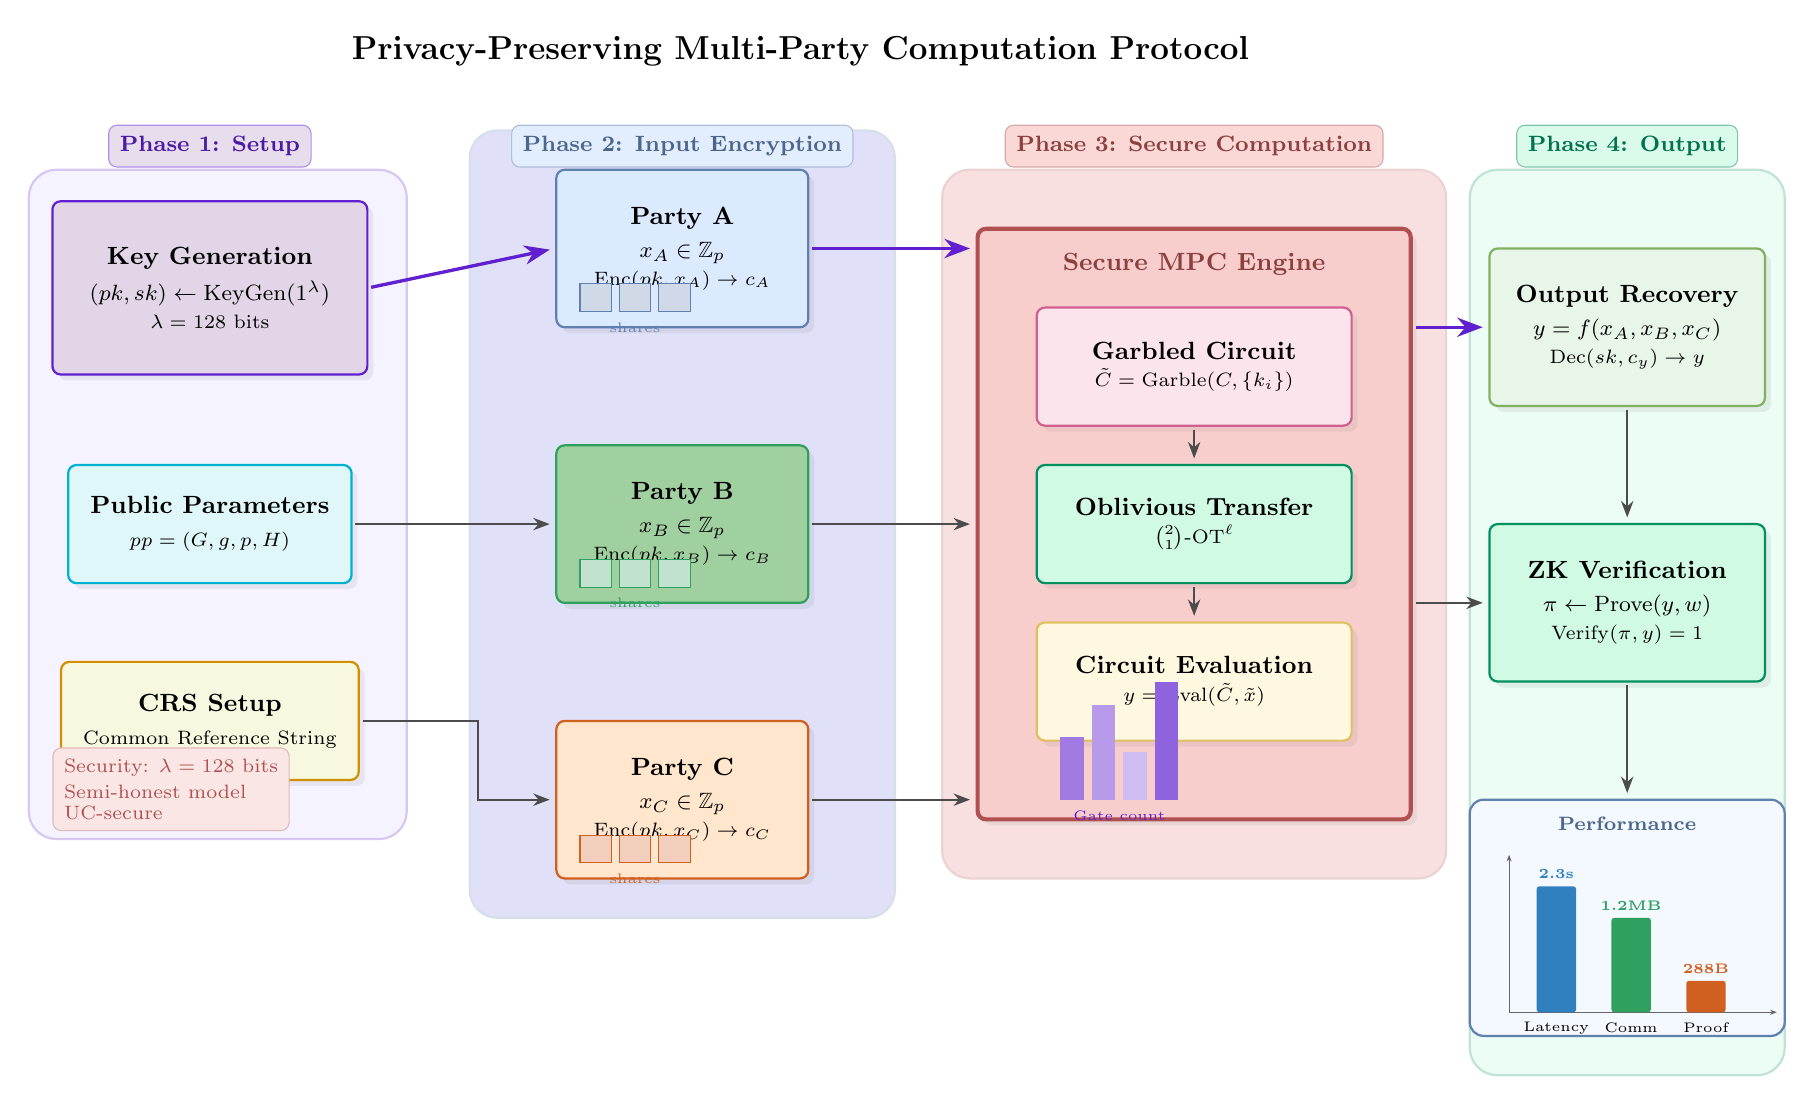
\begin{tikzpicture}[
    every node/.style={font=\small},
    base_box/.style={rectangle, rounded corners=3pt, align=center,
        minimum height=0.9cm, minimum width=2.6cm,
        inner sep=8pt, drop shadow={opacity=0.12}, thick},
    blue_node/.style={base_box, fill=acaBlueFill, draw=acaBlueLine},
    green_node/.style={base_box, fill=acaGreenFill, draw=acaGreenLine},
    orange_node/.style={base_box, fill=acaOrangeFill, draw=acaOrangeLine},
    purple_node/.style={base_box, fill=acaPurpleFill, draw=acaPurpleLine},
    red_node/.style={base_box, fill=acaRedFill, draw=acaRedLine, font=\small\bfseries},
    grey_node/.style={base_box, fill=acaGreyFill, draw=acaGreyLine},
    gold_node/.style={base_box, fill=acaGoldFill, draw=acaGoldLine},
    teal_node/.style={base_box, fill=acaTealFill, draw=acaTealLine},
    cyan_node/.style={base_box, fill=acaCyanFill, draw=acaCyanLine},
    pink_node/.style={base_box, fill=acaPinkFill, draw=acaPinkLine},
    yellow_node/.style={base_box, fill=acaYellowFill, draw=acaYellowLine},
    lime_node/.style={base_box, fill=acaLimeFill, draw=acaLimeLine},
    arrow/.style={-{Stealth[scale=0.9]}, thick, color=black!70, shorten >=2pt, shorten <=1pt},
    data_arrow/.style={-{Stealth[scale=1.1]}, very thick, color=acaPurpleLine, shorten >=2pt, shorten <=1pt},
]

% ================================================================
%  Title
% ================================================================
\node[font=\large\bfseries] at (10, 17.5)
    {Privacy-Preserving Multi-Party Computation Protocol};

% ================================================================
%  Phase 1: Key Generation (x=0~5)
% ================================================================
\node[purple_node, minimum width=4cm, minimum height=2.2cm] (keygen) at (2.5, 14.5)
    {\textbf{Key Generation}\\[2pt]{\footnotesize $(pk, sk) \leftarrow \mathrm{KeyGen}(1^\lambda)$}\\[-1pt]{\scriptsize $\lambda = 128$ bits}};

\node[cyan_node, minimum width=3.5cm, minimum height=1.5cm] (params) at (2.5, 11.5)
    {\textbf{Public Parameters}\\[1pt]{\scriptsize $pp = (G, g, p, H)$}};

\node[gold_node, minimum width=3.5cm, minimum height=1.5cm] (crs) at (2.5, 9.0)
    {\textbf{CRS Setup}\\[1pt]{\scriptsize Common Reference String}};

% ================================================================
%  Phase 2: Encryption & Secret Sharing (x=6~12)
% ================================================================
% Party A
\node[blue_node, minimum width=3.2cm, minimum height=2.0cm] (partyA) at (8.5, 15.0)
    {\textbf{Party A}\\[1pt]{\footnotesize $x_A \in \mathbb{Z}_p$}\\[-1pt]{\scriptsize Enc$(pk, x_A) \to c_A$}};
% Party B
\node[green_node, minimum width=3.2cm, minimum height=2.0cm] (partyB) at (8.5, 11.5)
    {\textbf{Party B}\\[1pt]{\footnotesize $x_B \in \mathbb{Z}_p$}\\[-1pt]{\scriptsize Enc$(pk, x_B) \to c_B$}};
% Party C
\node[orange_node, minimum width=3.2cm, minimum height=2.0cm] (partyC) at (8.5, 8.0)
    {\textbf{Party C}\\[1pt]{\footnotesize $x_C \in \mathbb{Z}_p$}\\[-1pt]{\scriptsize Enc$(pk, x_C) \to c_C$}};

% Secret sharing visualization (small matrix inside each party)
\foreach \party/\ybase/\col in {A/14.2/acaBlueLine, B/10.7/acaGreenLine, C/7.2/acaOrangeLine} {
  \foreach \s in {0,1,2} {
    \fill[\col!30] ({7.2+\s*0.5}, \ybase) rectangle ({7.2+\s*0.5+0.4}, {\ybase+0.35});
    \draw[\col, thin] ({7.2+\s*0.5}, \ybase) rectangle ({7.2+\s*0.5+0.4}, {\ybase+0.35});
  }
  \node[font=\tiny, text=\col] at (7.9, {\ybase-0.2}) {shares};
}

% ================================================================
%  Phase 3: Secure Computation (x=13~18) — Core
% ================================================================
\node[red_node, minimum width=5.5cm, minimum height=7.5cm, line width=1.5pt] (mpc) at (15, 11.5) {};
\node[font=\small\bfseries, text=acaRedLine!80!black] at (15, 14.8) {Secure MPC Engine};

% Garbled Circuit inside
\node[pink_node, minimum width=4.0cm, minimum height=1.5cm] (garbled) at (15, 13.5)
    {\textbf{Garbled Circuit}\\[-1pt]{\scriptsize $\tilde{C} = \mathrm{Garble}(C, \{k_i\})$}};

% OT (Oblivious Transfer)
\node[teal_node, minimum width=4.0cm, minimum height=1.5cm] (ot) at (15, 11.5)
    {\textbf{Oblivious Transfer}\\[-1pt]{\scriptsize $\binom{2}{1}\text{-OT}^\ell$}};

% Evaluation
\node[yellow_node, minimum width=4.0cm, minimum height=1.5cm] (eval) at (15, 9.5)
    {\textbf{Circuit Evaluation}\\[-1pt]{\scriptsize $y = \mathrm{Eval}(\tilde{C}, \tilde{x})$}};

% Internal arrows
\draw[arrow] (garbled.south) -- (ot.north);
\draw[arrow] (ot.south) -- (eval.north);

% Embedded gate count mini-chart
% Fix F.3: was shift=(13.3, 7.8) with label at y=7.6 — outside Phase 3
% core box bottom y=7.75. Moved up to (13.3, 8.0) so label at y=7.8 is
% just above box bottom (7.75) — fully inside.
\begin{scope}[shift={(13.3, 8.0)}]
  \fill[acaPurpleLine!60] (0.0, 0) rectangle (0.3, 0.8);
  \fill[acaPurpleLine!45] (0.4, 0) rectangle (0.7, 1.2);
  \fill[acaPurpleLine!30] (0.8, 0) rectangle (1.1, 0.6);
  \fill[acaPurpleLine!70] (1.2, 0) rectangle (1.5, 1.5);
  \node[font=\tiny, text=acaPurpleLine] at (0.75, -0.2) {Gate count};
\end{scope}

% ================================================================
%  Phase 4: Output & Verification (x=19~23)
% ================================================================
\node[lime_node, minimum width=3.5cm, minimum height=2.0cm] (output) at (20.5, 14.0)
    {\textbf{Output Recovery}\\[1pt]{\footnotesize $y = f(x_A, x_B, x_C)$}\\[-1pt]{\scriptsize Dec$(sk, c_y) \to y$}};

\node[teal_node, minimum width=3.5cm, minimum height=2.0cm] (verify) at (20.5, 10.5)
    {\textbf{ZK Verification}\\[1pt]{\footnotesize $\pi \leftarrow \mathrm{Prove}(y, w)$}\\[-1pt]{\scriptsize $\mathrm{Verify}(\pi, y) = 1$}};

% Performance panel
\node[rectangle, rounded corners=5pt, draw=acaBlueLine, fill=acaBlueFill!30,
      minimum width=4.0cm, minimum height=3.0cm, thick] (perf) at (20.5, 6.5) {};
\node[font=\scriptsize\bfseries, text=acaBlueLine!80!black] at (20.5, 7.7) {Performance};

% Mini bar chart — wider bar spacing (0.95cm) so "Latency" label
% doesn't overlap "Comm" / "Proof" labels (was 0.7cm gap → overlap)
\begin{scope}[shift={(18.8, 5.3)}]
  \draw[-{Stealth[scale=0.5]}, acaGreyLine] (0.2, 0) -- (0.2, 2.0);
  \draw[-{Stealth[scale=0.5]}, acaGreyLine] (0.2, 0) -- (3.6, 0);
  \fill[barBlue, rounded corners=1pt] (0.55, 0) rectangle (1.05, 1.6);
  \fill[barGreen, rounded corners=1pt] (1.50, 0) rectangle (2.00, 1.2);
  \fill[barOrange, rounded corners=1pt] (2.45, 0) rectangle (2.95, 0.4);
  \node[font=\tiny] at (0.8, -0.2) {Latency};
  \node[font=\tiny] at (1.75, -0.2) {Comm};
  \node[font=\tiny] at (2.7, -0.2) {Proof};
  \node[font=\tiny\bfseries, text=barBlue] at (0.8, 1.75) {2.3s};
  \node[font=\tiny\bfseries, text=barGreen] at (1.75, 1.35) {1.2MB};
  \node[font=\tiny\bfseries, text=barOrange] at (2.7, 0.55) {288B};
\end{scope}

% ================================================================
%  CONNECTIONS
% ================================================================
% Phase 1 → Phase 2
\draw[data_arrow] (keygen.east) -- (partyA.west);
\draw[arrow] (params.east) -- ++(1.5, 0) |- (partyB.west);
\draw[arrow] (crs.east) -- ++(1.5, 0) |- (partyC.west);

% Phase 2 → Phase 3
\draw[data_arrow, rounded corners=6pt] (partyA.east) -- (mpc.west |- partyA);
\draw[arrow, rounded corners=6pt] (partyB.east) -- (mpc.west |- partyB);
\draw[arrow, rounded corners=6pt] (partyC.east) -- (mpc.west |- partyC);

% Phase 3 → Phase 4
\draw[data_arrow, rounded corners=6pt] (mpc.east |- output) -- (output.west);
\draw[arrow, rounded corners=6pt] (mpc.east |- verify) -- (verify.west);

% Output → Verify
\draw[arrow] (output.south) -- (verify.north);

% Verify → Performance
\draw[arrow] (verify.south) -- (perf.north);

% ================================================================
%  ZONE BACKGROUNDS
% ================================================================
\begin{pgfonlayer}{background}
  \fill[zonePurpleBg, rounded corners=10pt] (0.2, 7.5) rectangle (5.0, 16.0);
  \draw[acaPurpleLine!25, thick, rounded corners=10pt] (0.2, 7.5) rectangle (5.0, 16.0);

  \fill[zoneBlueBg, rounded corners=10pt] (5.8, 6.5) rectangle (11.2, 16.5);
  \draw[acaBlueLine!25, thick, rounded corners=10pt] (5.8, 6.5) rectangle (11.2, 16.5);

  \fill[zoneRedBg, rounded corners=10pt] (11.8, 7.0) rectangle (18.2, 16.0);
  \draw[acaRedLine!25, thick, rounded corners=10pt] (11.8, 7.0) rectangle (18.2, 16.0);

  \fill[zoneGreenBg, rounded corners=10pt] (18.5, 4.5) rectangle (22.5, 16.0);
  \draw[acaTealLine!25, thick, rounded corners=10pt] (18.5, 4.5) rectangle (22.5, 16.0);
\end{pgfonlayer}

% ================================================================
%  PHASE LABELS
% ================================================================
\node[font=\footnotesize\bfseries, fill=acaPurpleFill!80, draw=acaPurpleLine!50,
      rounded corners=3pt, inner sep=4pt, text=acaPurpleLine!80!black]
      at (2.5, 16.3) {Phase 1: Setup};
\node[font=\footnotesize\bfseries, fill=acaBlueFill!80, draw=acaBlueLine!50,
      rounded corners=3pt, inner sep=4pt, text=acaBlueLine!80!black]
      at (8.5, 16.3) {Phase 2: Input Encryption};   % Fix F.2: was 16.8 → 0.5cm higher than other 3 phase chips
\node[font=\footnotesize\bfseries, fill=acaRedFill!80, draw=acaRedLine!50,
      rounded corners=3pt, inner sep=4pt, text=acaRedLine!80!black]
      at (15, 16.3) {Phase 3: Secure Computation};
\node[font=\footnotesize\bfseries, fill=acaTealFill!80, draw=acaTealLine!50,
      rounded corners=3pt, inner sep=4pt, text=acaTealLine!80!black]
      at (20.5, 16.3) {Phase 4: Output};

% ================================================================
%  SECURITY ANNOTATION
% ================================================================
% Fix F.1: Security note was anchor=north west at (0.5, 7.2) — outside
% Phase 1 zone bottom (y=7.5). Move INTO Phase 1 zone bottom area:
% anchor=south west at (0.5, 7.6) places note at bottom of Phase 1 zone.
\node[font=\scriptsize, text=acaRedLine, fill=acaRedFill!50, draw=acaRedLine!40,
      rounded corners=3pt, inner sep=4pt, anchor=south west] at (0.5, 7.6)
    {\shortstack[l]{Security: $\lambda = 128$ bits\\Semi-honest model\\UC-secure}};

\end{tikzpicture}
\end{document}
